%* 
%* ------------------------------------------------------------------
%* TimeTable.tex - Time Table Manual
%* Created by Robert Heller on Tue Aug  4 14:05:46 2009
%* ------------------------------------------------------------------
%* Modification History: $Log$
%* Modification History: Revision 1.1  2002/07/28 14:03:50  heller
%* Modification History: Add it copyright notice headers
%* Modification History:
%* ------------------------------------------------------------------
%* Contents:
%* ------------------------------------------------------------------
%*  
%*     Model RR System, Version 2
%*     Copyright (C) 1994,1995,2002-2005  Robert Heller D/B/A Deepwoods Software
%* 			51 Locke Hill Road
%* 			Wendell, MA 01379-9728
%* 
%*     This program is free software; you can redistribute it and/or modify
%*     it under the terms of the GNU General Public License as published by
%*     the Free Software Foundation; either version 2 of the License, or
%*     (at your option) any later version.
%* 
%*     This program is distributed in the hope that it will be useful,
%*     but WITHOUT ANY WARRANTY; without even the implied warranty of
%*     MERCHANTABILITY or FITNESS FOR A PARTICULAR PURPOSE.  See the
%*     GNU General Public License for more details.
%* 
%*     You should have received a copy of the GNU General Public License
%*     along with this program; if not, write to the Free Software
%*     Foundation, Inc., 675 Mass Ave, Cambridge, MA 02139, USA.
%* 
%*  
%* 

\documentclass[12pt,notitlepage,twoside]{book}
\usepackage{graphicx}
\usepackage{mathptm}
\usepackage{times}
\usepackage{makeidx}
\usepackage{url}
\usepackage{supertabular}
\usepackage{MyTitlepage}
\usepackage{listings}
\pagestyle{headings}
\makeindex
\emergencystretch=50pt
\begin{document}
\lstset{language=Tcl,basicstyle=\footnotesize,numbers=left,stepnumber=5}% Most examples will be in Tcl
\newcommand{\MRRSubTitle}{Time Table Manual}
%* 
%* ------------------------------------------------------------------
%* titlepage.tex - Common documentation title page
%* Created by Robert Heller on Sun Oct 13 15:59:49 2002
%* ------------------------------------------------------------------
%* Modification History: $Log$
%* Modification History: Revision 1.3  2007/10/22 17:17:27  heller
%* Modification History: 10222007
%* Modification History:
%* Modification History: Revision 1.2  2004/04/14 23:20:24  heller
%* Modification History: Updated copyright.
%* Modification History:
%* Modification History: Revision 1.1  2002/10/17 00:02:24  heller
%* Modification History: Documentation support files.
%* Modification History:
%* Modification History: Revision 1.1  2002/07/28 14:03:50  heller
%* Modification History: Add it copyright notice headers
%* Modification History:
%* ------------------------------------------------------------------
%* Contents:
%* ------------------------------------------------------------------
%*  
%*     Model RR System, Version 2
%*     Copyright (C) 1994,1995,2002  Robert Heller D/B/A Deepwoods Software
%* 			51 Locke Hill Road
%* 			Wendell, MA 01379-9728
%* 
%*     This program is free software; you can redistribute it and/or modify
%*     it under the terms of the GNU General Public License as published by
%*     the Free Software Foundation; either version 2 of the License, or
%*     (at your option) any later version.
%* 
%*     This program is distributed in the hope that it will be useful,
%*     but WITHOUT ANY WARRANTY; without even the implied warranty of
%*     MERCHANTABILITY or FITNESS FOR A PARTICULAR PURPOSE.  See the
%*     GNU General Public License for more details.
%* 
%*     You should have received a copy of the GNU General Public License
%*     along with this program; if not, write to the Free Software
%*     Foundation, Inc., 675 Mass Ave, Cambridge, MA 02139, USA.
%* 
%*  
%* 
%* 
%* $Id$  
%* 

\title{Model Railroad System \\ A collection of utilities for Model Railroaders\\ \MRRSubTitle}
\author{Robert Heller \\ Deepwoods Software \\ Wendell, MA, USA}
\date{\today}
\begin{titlepage}

\maketitle

%\begin{centering}
%\epsfig{file=../Cover1.ps} \\
%\end{centering}

\clearpage


This documentation was prepared with \LaTeX.

This document describes version 2 of the Model Railroad System package.

\vspace{.25in}



{\small Copyright \copyright 1994,1995,2002-2012 by Robert Heller D/B/A Deepwoods
Software}

\vspace{.25in}

All rights reserved.  Permission is granted to copy this document in
electronic form only, so long as it is with the software it
documents. 

The author, Robert Heller, may be contacted electronically (E-Mail) via
the following:

\begin{description}
\item[FidoNet] 1:321/153, Locks Hill BBS.
\item[InterNet] heller@deepsoft.com
\end{description}

Web site URL: {\tt http://www.deepsoft.com/}.

\thispagestyle{empty}
\setcounter{page}{0}
\clearpage

\end{titlepage}


\pagenumbering{roman}
\tableofcontents
\listoffigures
\listoftables
\cleardoublepage
%       
%%* 
%* ------------------------------------------------------------------
%* Preface.tex - Preface to the user manual
%* Created by Robert Heller on Sat Apr 21 10:32:44 2007
%* ------------------------------------------------------------------
%* Modification History: $Log$
%* Modification History: Revision 1.1  2007/05/06 12:49:40  heller
%* Modification History: Lock down  for 2.1.8 release candidate 1
%* Modification History:
%* Modification History: Revision 1.1  2002/07/28 14:03:50  heller
%* Modification History: Add it copyright notice headers
%* Modification History:
%* ------------------------------------------------------------------
%* Contents:
%* ------------------------------------------------------------------
%*  
%*     Model RR System, Version 2
%*     Copyright (C) 1994,1995,2002-2005  Robert Heller D/B/A Deepwoods Software
%* 			51 Locke Hill Road
%* 			Wendell, MA 01379-9728
%* 
%*     This program is free software; you can redistribute it and/or modify
%*     it under the terms of the GNU General Public License as published by
%*     the Free Software Foundation; either version 2 of the License, or
%*     (at your option) any later version.
%* 
%*     This program is distributed in the hope that it will be useful,
%*     but WITHOUT ANY WARRANTY; without even the implied warranty of
%*     MERCHANTABILITY or FITNESS FOR A PARTICULAR PURPOSE.  See the
%*     GNU General Public License for more details.
%* 
%*     You should have received a copy of the GNU General Public License
%*     along with this program; if not, write to the Free Software
%*     Foundation, Inc., 675 Mass Ave, Cambridge, MA 02139, USA.
%* 
%*  
%* 

\chapter*{Preface}
\markboth{PREFACE}{PREFACE}%
\addcontentsline{toc}{chapter}{Preface}
\label{chpt:Preface}
\typeout{$Id$}

This is the user manual for the Model Railroad system.  It is a ``work
in progress'' and I will be adding chapters as I write the various
self-contained ``main programs''.

%
\cleardoublepage
\pagenumbering{arabic}
%
%%* 
%* ------------------------------------------------------------------
%* Introduction.tex - Introduction
%* Created by Robert Heller on Thu Apr 19 14:24:42 2007
%* ------------------------------------------------------------------
%* Modification History: $Log$
%* Modification History: Revision 1.1  2007/05/06 12:49:38  heller
%* Modification History: Lock down  for 2.1.8 release candidate 1
%* Modification History:
%* Modification History: Revision 1.1  2002/07/28 14:03:50  heller
%* Modification History: Add it copyright notice headers
%* Modification History:
%* ------------------------------------------------------------------
%* Contents:
%* ------------------------------------------------------------------
%*  
%*     Model RR System, Version 2
%*     Copyright (C) 1994,1995,2002-2005  Robert Heller D/B/A Deepwoods Software
%* 			51 Locke Hill Road
%* 			Wendell, MA 01379-9728
%* 
%*     This program is free software; you can redistribute it and/or modify
%*     it under the terms of the GNU General Public License as published by
%*     the Free Software Foundation; either version 2 of the License, or
%*     (at your option) any later version.
%* 
%*     This program is distributed in the hope that it will be useful,
%*     but WITHOUT ANY WARRANTY; without even the implied warranty of
%*     MERCHANTABILITY or FITNESS FOR A PARTICULAR PURPOSE.  See the
%*     GNU General Public License for more details.
%* 
%*     You should have received a copy of the GNU General Public License
%*     along with this program; if not, write to the Free Software
%*     Foundation, Inc., 675 Mass Ave, Cambridge, MA 02139, USA.
%* 
%*  
%* 

\chapter{Introduction}
\label{chapt:Introduction}
\typeout{$Id$}

This manual presents some information about how to write programs that
use various parts of Model Railroad System to control and manage various
aspects of operating your model railroad.  The Model Railroad System
includes code that interfaces with special hardware, including the PI
Engineering Raildriver Console (see
Chapter~\ref{chapt:RaildriverServer}), a Bruce Chubb network of control
nodes (see  Chapter~\ref{chapt:CMRIProgramming}), and a Lenz XPressNet
network (see Chapter~\ref{chapt:XPressNetProgramming}).  Also included
are a collection of Tcl scripts that implement a collection of widgets
that are useful for various aspects of programming utilities for a model
railroad system.

%* 
%* ------------------------------------------------------------------
%* TTTutorial.tex - Time Table (V2) Tutorial
%* Created by Robert Heller on Thu Apr 26 12:32:29 2007
%* ------------------------------------------------------------------
%* Modification History: $Log$
%* Modification History: Revision 1.1  2007/05/06 12:49:40  heller
%* Modification History: Lock down  for 2.1.8 release candidate 1
%* Modification History:
%* Modification History: Revision 1.1  2002/07/28 14:03:50  heller
%* Modification History: Add it copyright notice headers
%* Modification History:
%* ------------------------------------------------------------------
%* Contents:
%* ------------------------------------------------------------------
%*  
%*     Model RR System, Version 2
%*     Copyright (C) 1994,1995,2002-2005  Robert Heller D/B/A Deepwoods Software
%* 			51 Locke Hill Road
%* 			Wendell, MA 01379-9728
%* 
%*     This program is free software; you can redistribute it and/or modify
%*     it under the terms of the GNU General Public License as published by
%*     the Free Software Foundation; either version 2 of the License, or
%*     (at your option) any later version.
%* 
%*     This program is distributed in the hope that it will be useful,
%*     but WITHOUT ANY WARRANTY; without even the implied warranty of
%*     MERCHANTABILITY or FITNESS FOR A PARTICULAR PURPOSE.  See the
%*     GNU General Public License for more details.
%* 
%*     You should have received a copy of the GNU General Public License
%*     along with this program; if not, write to the Free Software
%*     Foundation, Inc., 675 Mass Ave, Cambridge, MA 02139, USA.
%* 
%*  
%* 

\chapter{Time Table (V2) Tutorial}
\label{chpt:tt:Tutorial}
\typeout{$Id$}

\index{Time Table!Tutorial|(} The Time Table is a program designed to
create railroad employee timetables.  The program's main display is a
graph of time (of day) versus distance (along the railroad), gridded at
time intervals and at station stops.  Trains schedules are represented
as colored lines on this graph, with diagonals representing train
movement at speed and horizontal lines representing trains ``siting''
at stations (layovers or switching).

\section{Creating a new time table}

To create an new time table select the \verb=File->New= menu item or
the 
\includegraphics{TTNewTool.png} toolbar button. A ``Create a New
Time Table'' dialog, described in
Section~\ref{sect:tt:createnewtimetable}. is displayed.  This dialog
box collects three pieces of information: the name of the new time
table, the total time (in minutes) the time table will cover (there are
1440 minutes in a 24 hour day), and the tick interval in minutes.  A
new time table can also me created from the command line by including
the options \verb=-totaltime= and \verb=-timeincrement= along with a
name for the new time table.

\subsection{Creating stations}

Once the name and the two time elements have been selected, a set of at
least two stations need to be created.  This is done with the ``Create
All Stations Dialog'',  described in
Section~\ref{sect:tt:CreateAllStationsDialog}.  This dialog box is
used to create stations, which can have zero or more storage tracks. 
Storage tracks are used when a train has a long layover (and needs to
be ``out of the way'' of other traffic) or when a train terminates and
the train set is re-used for a different schedule, generally in the
opposite direction. As the stations and their storage tracks are
created, they are displayed in the station listing in the upper part of
the dialog. 

\subsection{Creating cabs}

After creating all of the stations, zero or more cabs can be created. 
Cabs are mostly for switched block DC layouts, but creating ``cabs''
for a DCC layout is useful, since it allows for a way to visually group
trains operationally. Think of the cabs as a way of defining ``crews''
(operators).  This allows for things like crew (operator) changes as
the train moves to different parts of the layout for example.

\section{Creating trains}

Once the stations and cabs have been created, the program displays an
empty chart.  The chart's \verb=x= axis is time (in minutes).  The upper
section of the chart has the cabs (if any), the middle part of the chart
has the stations, and the bottom part of the chart has the storage
tracks (if any).  Now we can create a train.  This is done by selecting
either the \verb=Trains->Add Train= menu item, clicking on the add train
(
\includegraphics{TTaddtrain.png}) toolbar button or the 
\verb=Add a new train= button.  All of these display the ``Create New
Train Dialog'', described in Section~\ref{sect:tt:CreateNewTrainDialog}.

Trains have a (common) name, a number (or symbol), a class number, an average
speed, a scheduled departure time, and travel between two stations.  The
train's number (or symbol) needs to be a unique identification of the
train. The class is a whole number, with smaller numbers generally being
the ``higher'' class.  The class is used to indicate a train's priority
and is also used to group similar trains together.  The speed is the
(scale) speed the train will be traveling between stops.  The scheduled
departure time is the time the train is scheduled to leave its origin
station.  The origin and termination stations are the station end points
the train travels between.  The train will get a ``stop'' at every
intermediate station between these two stations.  Note that the train
won't be expected to actually stop at any station where the layover time
is set to zero.  Such stops would just be timekeeping points.

Once the train's basic information is set, the \verb=Schedule= button can be
clicked.  This shifts to the schedule page, where layovers and cab
assignments cab be set.  The \verb=Update= buttons propagate the
cab settings and adjust the times to allow for the layovers.  If the
train makes use of station storage tracks, the \verb=Storage= button can
be clicked and storage tracks selected.  When the train is fully
configured, the \verb=Done= button can be clicked to actually create the
train.

\section{Printing a time table}

Once all of the trains have been added, it it possible to ``print'' a
timetable.  The LaTeX system is used to format the time table and the
TimeTable program generates a \LaTeX{} source file (\verb=.tex=) and will
run the \LaTeX{} program, \verb=pdflatex=, to create a PDF file from the
\LaTeX{} source file.  This process is started with the
\verb=File->Print...= menu item or the
\includegraphics{TTprintTool.png} toolbar button.  This pops up the
``Print Dialog'', described in Section~\ref{sect:tt:PrintTimetableDialog}.
This dialog collects the name of the \LaTeX{} source file, and the path to the
\LaTeX{} processing programing, as well as a few other options.  It also
has a button to configure how the timetable will be formatted.  

The \verb=Configure= button pops up the ``Print Configuration Dialog'',
described in Section~\ref{sect:tt:PrintConfigurationDialog}, which has
three sections, a \verb=General= section which gets some general
configuration settings, a \verb=Multi= section for various
configuration settings relating to printing multiple tables, and a
\verb=Groups= section, for configuring groups of trains.  Some of the
configuration assumes some knowledge of \LaTeX. A visit to the \TeX{} and
\LaTeX{} web pages (\url{http://www.tug.org}) is a good place to start,
with the beginner's page at \url{http://www.tug.org/begin.html} as the
obvious starting point.  You don't really have to learn how to use
\LaTeX{}, you just need to have a \TeX/\LaTeX{} system installed.  The only
other issue is the \verb=TimeTable.sty= file.  This file either needs to be
installed somewhere in the \TeX/\LaTeX{} search path or it needs to be in
the same directory as the \LaTeX{} source file generated by the TimeTable
program. You will need to learn a little about \LaTeX{} if you want to
include various sorts of customizations.
\index{Time Table!Tutorial|)} 

%* 
%* ------------------------------------------------------------------
%* TTReference.tex - Time Table (V2) Reference
%* Created by Robert Heller on Thu Apr 26 12:33:54 2007
%* ------------------------------------------------------------------
%* Modification History: $Log$
%* Modification History: Revision 1.1  2007/05/06 12:49:40  heller
%* Modification History: Lock down  for 2.1.8 release candidate 1
%* Modification History:
%* Modification History: Revision 1.1  2002/07/28 14:03:50  heller
%* Modification History: Add it copyright notice headers
%* Modification History:
%* ------------------------------------------------------------------
%* Contents:
%* ------------------------------------------------------------------
%*  
%*     Model RR System, Version 2
%*     Copyright (C) 1994,1995,2002-2005  Robert Heller D/B/A Deepwoods Software
%* 			51 Locke Hill Road
%* 			Wendell, MA 01379-9728
%* 
%*     This program is free software; you can redistribute it and/or modify
%*     it under the terms of the GNU General Public License as published by
%*     the Free Software Foundation; either version 2 of the License, or
%*     (at your option) any later version.
%* 
%*     This program is distributed in the hope that it will be useful,
%*     but WITHOUT ANY WARRANTY; without even the implied warranty of
%*     MERCHANTABILITY or FITNESS FOR A PARTICULAR PURPOSE.  See the
%*     GNU General Public License for more details.
%* 
%*     You should have received a copy of the GNU General Public License
%*     along with this program; if not, write to the Free Software
%*     Foundation, Inc., 675 Mass Ave, Cambridge, MA 02139, USA.
%* 
%*  
%* 

\chapter{Time Table (V2) Reference}
\label{chpt:tt:Reference}
\typeout{$Id$}

The Time Table (V2) program is a hybrid program, consisting of a Tcl/Tk
GUI on top of a C++ class library.  The GUI provides the user interface
to the algorithms and data structures contained in the C++ class
library.  This program was inspired by chapter 8 of the book {\it How
to Operate Your Model Railroad}\cite{Chubb77} by Bruce A. Chubb.  I
strongly recommend reading this chapter fully before using this
program.  This program implements the methods described in this
chapter, in an automated fashion.

\section{Command Line Usage}

\begin{figure}[hbpt] 
\begin{centering} 
{\footnotesize
\begin{verbatim} 
TimeTable oldtimetablefile 
TimeTable -totaltime time -timeincrement time nameoftimetable 
\end{verbatim} 
}
\caption{Command Line Format for the TimeTable command} 
\label{fig:tt:cliusage} 
\end{centering} 
\end{figure}
There are two formats for the TimeTable program's command line.  The
command line can either have a single file name, the name of an
existing time table file or it can have two options (\texttt{-totaltime}
and \texttt{-timeincrement}) and the name of a new time table.  The first
form loads an existing time table (see
Section~\ref{sect:tt:loadexistingtimetable} and the second form creates
a new time table (see Section~\ref{sect:tt:createnewtimetable}.  These
two command line formats are shown in Figure~\ref{fig:tt:cliusage}. 

\section{Layout of the Main GUI}

\begin{figure}[hbpt]
\begin{centering}
\includegraphics[width=5in]{TTMainGUIBlank.png}
\caption{The main GUI screen of the Time Table (V2) Program}
\label{fig:tt:MainGUIBlank}
\end{centering}
\end{figure}
\begin{figure}[hbpt]
\begin{centering}
\includegraphics[width=5in]{TTMainGUIToolBar.png}
\caption{The Toolbar of the Time Table (V2) Program}
\label{fig:tt:MainGUIToolBar}
\end{centering}
\end{figure}
\begin{figure}[hbpt]
\begin{centering}
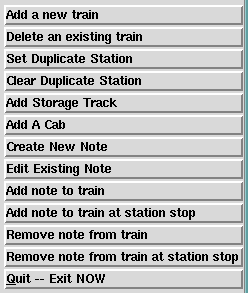
\includegraphics{TTMainGUIButtonMenu.png}
\caption{The Button Menu of the Time Table (V2) Program}
\label{fig:tt:MainGUIButtonMenu}
\end{centering}
\end{figure}
The main GUI window\index{Time Table!main GUI}, show in
Figure~\ref{fig:tt:MainGUIBlank}, contains a menu bar, a toolbar
(Figure~\ref{fig:tt:MainGUIToolBar}), a time table chart, and a button
menu (Figure~\ref{fig:tt:MainGUIButtonMenu}).

\section{Creating a New Time Table}
\label{sect:tt:createnewtimetable}

\begin{figure}[hbpt]
\begin{centering}
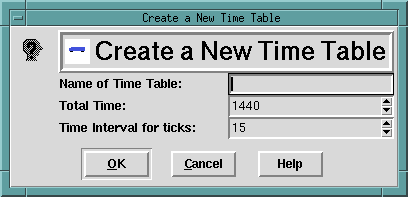
\includegraphics{TTCreateNewTT.png}
\caption{Create A New Time Table dialog}
\label{fig:tt:GetNewTimeTableDialog}
\end{centering}
\end{figure}
Creating a new time table can be done from the command line by
specifying a total time (in minutes) value with the \texttt{-totaltime}
option and a time increment value (in minutes) value with the
\texttt{-timeincrement} option and a name for the new time table (as
shown in the second line of Figure~\ref{fig:tt:cliusage}).  A new time
table can also be created with the \texttt{New} menu item of the
\texttt{File} menu or the

\includegraphics{TTNewTool.png} toolbar button. These later two methods
use the ``Create a New Time Table'' dialog, shown in
Figure~\ref{fig:tt:GetNewTimeTableDialog} to get the total time, time
increment, and the name of the new time table.  If there is a time
table file already loaded, a confirmation dialog will be displayed.

\subsection{Creating the station stops for a new time table}
\label{sect:tt:CreateAllStationsDialog}

\begin{figure}[hbpt]
\begin{centering}
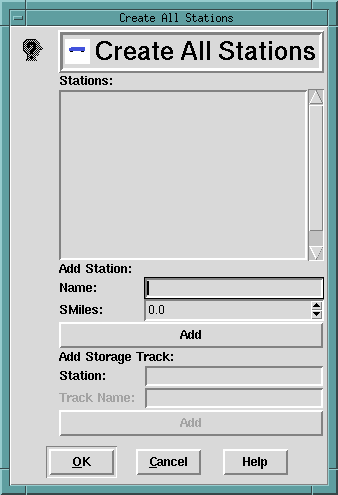
\includegraphics{TTCreateAllStations.png}
\caption{Create All Stations Dialog}
\label{fig:tt:CreateAllStationsDialog}
\end{centering}
\end{figure}
Stations for a time table must all be created when the time table is
created.  Stations cannot be added or removed later.  When a new time
table is created the ``Create All Stations Dialog'',  shown in
Figure~\ref{fig:tt:CreateAllStationsDialog} is displayed to create all
of the station stops.

\subsection{Creating an initial set of ``cabs''}

\begin{figure}[hbpt]
\begin{centering}
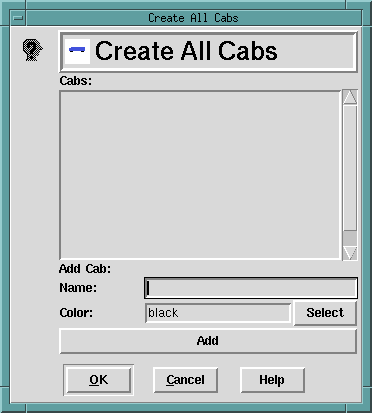
\includegraphics{TTCreateAllCabs.png}
\caption{Create All Cabs Dialog}
\label{fig:tt:CreateAllCabsDialog}
\end{centering}
\end{figure}
Once the stations have been created, an initial set of ``cabs'' can be
created.  Commonly, cabs are only used on block switch DC layouts, but
the cabs can be used as with a  DCC layout as a way to associate trains
with different operating ``crews'' (operators) or just to identify
different classes of trains by color, etc.  The ``Create All Cabs''
dialog, shown in Figure~\ref{fig:tt:CreateAllCabsDialog}, is used to
bulk create an initial set of cabs.

\begin{figure}[hbpt]
\begin{centering}   
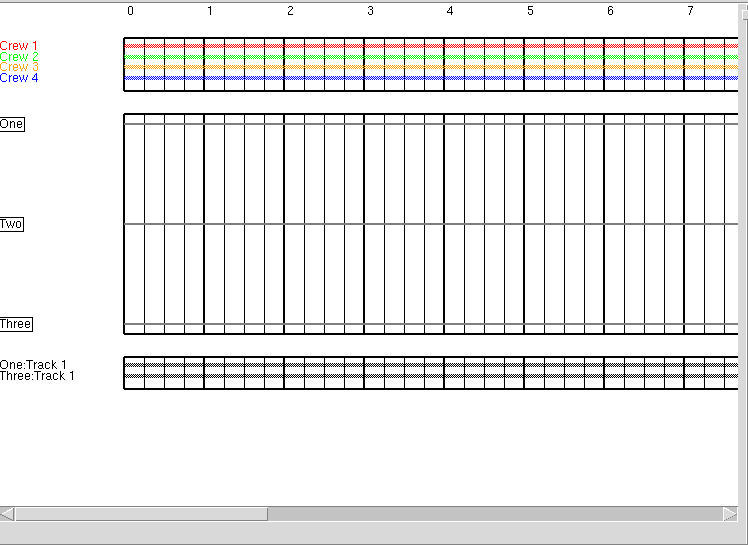
\includegraphics[width=5in]{TTChart3station.png}
\caption{Simple chart with three stations, four cabs, and two storage
tracks}
\label{fig:tt:Chart3station}
\end{centering}
\end{figure}   
A simple chart with three stations, four cabs (labeled ``Crew 1''
through ``Crew 4''), and two storage tracks is shown in
Figure~\ref{fig:tt:Chart3station}. 

\section{Loading an Exiting Time Table File}
\label{sect:tt:loadexistingtimetable}

An existing time table file can be loaded from the command line (as
shown in the first line of Figure~\ref{fig:tt:cliusage}),  with the
\texttt{Open...} menu item of the \texttt{File} menu or the

\includegraphics{TTOpenTool.png} toolbar button. If there is a time
table file already loaded, a confirmation dialog will be displayed.

\section{Saving a Time Table File}

The currently loaded time table can be saved with either the
\texttt{Save} (or \texttt{Save As...}) menu item of the \texttt{File} menu or
the \includegraphics{TTSaveTool.png} toolbar button. 

\section{Adding Trains}

Trains are added using the either the \texttt{Add Train} menu item of the
\texttt{Trains} menu, clicking on the add train
(
\includegraphics{TTaddtrain.png}) toolbar button or the \texttt{Add a
new train} button. All of these display the ``Create New Train
Dialog'', described in Section~\ref{sect:tt:CreateNewTrainDialog}.

\subsection{Create New Train Dialog}
\label{sect:tt:CreateNewTrainDialog}

\begin{figure}[hbpt]
\begin{centering}   
\includegraphics{TTCreateNewTrain1.png}
\caption{Creating a new train dialog, basic information}
\label{fig:tt:CreateNewTrain1}
\end{centering}
\end{figure}
The ``Create New Train Dialog'' first collects some basic information
about the new train, as shown in Figure~\ref{fig:tt:CreateNewTrain1}.
The basic train information consists of the train's common name, its
number (or symbol), its class number, its average speed, its scheduled
departure time, and the two stations it travels between.

The train's number (or symbol) needs to be a unique identification of
the train.  The common name need not be unique.  The class is a whole
number, with smaller numbers generally being the ``higher'' class. The
class is used to indicate a train's priority and is also used to group
similar trains together.  The speed is the (scale) speed the train will
be traveling between stops.  The scheduled departure time is the time
the train is scheduled to leave its origin station.  The origin and
termination stations are the station end points the train travels between.

\begin{figure}[hbpt]
\begin{centering}   
\includegraphics[width=5in]{TTCreateNewTrain2.png}
\caption{Creating a new train dialog, scheduling information}
\label{fig:tt:CreateNewTrain2}
\end{centering}
\end{figure}
The \texttt{Schedule} button selects the scheduling page of the ``Create a
New Train Dialog'', as shown in Figure~\ref{fig:tt:CreateNewTrain2}.  On
this page, the cab can be selected and layover periods at intermediate
stations can be set.  The \texttt{Update} buttons propagate the cab
settings and adjust the times to allow for the layovers.

\begin{figure}[hbpt]
\begin{centering}   
\includegraphics{TTCreateNewTrain3.png}
\caption{Creating a new train dialog, storage track selection}
\label{fig:tt:CreateNewTrain3}
\end{centering}
\end{figure}
The \texttt{Storage} button selects the storage track allocation page of
the ``Create a New Train Dialog'', as shown in
Figure~\ref{fig:tt:CreateNewTrain3}.  This page lists those stations
that have storage tracks available.  It only makes sense to select
storage tracks for intermediate stops if there is a layover or for
originating or terminating stops.

\section{Deleting Trains}
\label{sect:tt:DeletingTrains}

Trains are deleted using the \texttt{Delete Train} menu item of the
\texttt{Trains} menu, clicking on the delete train
(
\includegraphics{TTdeletetrain.png}) toolbar button or the
\texttt{Delete an Existing train} button. All of these display the
``Select One Train Dialog'', described in
Section~\ref{sect:tt:SelectOneTrainDialog}. A delete confirmation
dialog will also be displayed.

\section{Linking and Unlinking Duplicate Stations}

Duplicate stations occur mostly with ``out and back'' type layouts
where the opposite ends of the line are modeled with the same trackage
(usually a yard).  Duplicate stations also occur with reverse loops. In
all cases, these are stations which are logically different, but which
use the same tracks. There is an example in Figure~8-4 on page 86 of
\cite{Chubb77}. It is necessary to keep track of this trackage in the
schedule.  The duplicate station linking handles this. Duplicate
stations need to be setup before trains have been added.

The \texttt{Set Duplicate Station} and 
\texttt{Clear Duplicate Station} menu items of the \texttt{Stations} menu, the
\includegraphics{TTsetdupstation.png} and

\includegraphics{TTcleardupstation.png} toolbar buttons, and the
\texttt{Set Duplicate Station} and \texttt{Clear Duplicate Station} buttons
set and clear duplicate stations.

\section{Adding Station Storage Tracks}

Storage tracks are sidings where whole trains can be stored, either
during a long layover or between trips. The  \texttt{Add Storage Track}
menu item of the \texttt{Stations} menu, the

\includegraphics{TTaddstorage.png} toolbar button, or the  \texttt{Add
Storage Track} button are used to add a storage track to a station.

\section{Adding Cabs}

Generally ``Cabs'' refer to the separate throttle controls on a block
switched DC layout.  They are generally non-existent with a DCC layout,
but virtual cabs might be used as a way of assigning crews (operators)
to a train or to a segment of a train's run.  Cabs are added with the
\texttt{Add A Cab} menu item of the \texttt{Cabs} menu, the

\includegraphics{TTaddcab.png} toolbar button or the \texttt{Add A Cab}
button.

\section{Handling Notes}

Notes are brief memos about the operating rules in effect.  There is a
single pool of notes.  Notes from this pool can be associated either
with a whole train or with a train at a station stop.  The notes can
specify schedule exceptions (eg ``Daily except Saturdays, Sundays, and
Holidays''), or operating rules relating to meets.

\subsection{Creating New Notes and Editing Existing Notes}

\begin{figure}[hbpt]
\begin{centering}   
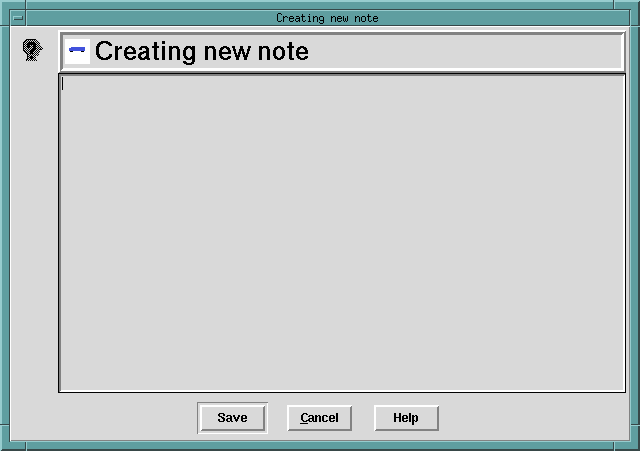
\includegraphics[width=5in]{TTEditNote.png}
\caption{Note editor dialog}
\label{fig:tt:EditNote}
\end{centering}
\end{figure}
Notes are created and edited the \texttt{Create New Note} and
\texttt{Edit Existing Note} menu items of the \texttt{Notes} menu, the

\includegraphics{TTcreatenote.png} and \includegraphics{TTeditnote.png}
toolbar buttons, or the \texttt{Create New Note} and 
\texttt{Edit Existing Note} buttons.  The the ``Note editor dialog'', shown in
Figure~\ref{fig:tt:EditNote} is used to create or edit the note.  Notes are
numbered consecutively starting with 1.

\subsection{Adding and Removing a Notes To Trains}

\begin{figure}[hbpt]
\begin{centering}
\includegraphics{TTAddNote.png}
\caption{Add (or Remove) Note dialog}
\label{fig:tt:AddNote}
\end{centering}
\end{figure}
Notes are added to trains or removed from trains with \texttt{Notes} menu
items \texttt{Add note to train}, \texttt{Add note to train at station stop},
\texttt{Remove note from train}, and 
\texttt{Remove note from train at station stop}; the
\includegraphics{TTaddnotetotrain.png},
\includegraphics{TTaddnotetotrainatstation.png},
\includegraphics{TTremovenotefromtrain.png}, and

\includegraphics{TTremovenotefromtrainatstation.png}; or the  
\texttt{Add note to train}, \texttt{Add note to train at station stop}, 
\texttt{Remove note from train}, and 
\texttt{Remove note from train at station stop} buttons.  All of these
display the ``Add (or Remove) Note dialog'', shown in
Figure~\ref{fig:tt:AddNote}.

\section{Printing a Time Table}

``Printing'' a time table actually means creating a \LaTeX{} file and
then processing that \LaTeX{} file through a \LaTeX{} processing program
(typically \texttt{pdflatex}).  \LaTeX{} provides the means to produce a
professionally formatted document and has the means to provide things
like table of contents and the creation of a final document in a
selection of different final formats, including PDF (via
\texttt{pdflatex}), PostScript (via \texttt{latex} and \texttt{dvips})
or HTML (via the \texttt{htlatex} script from \textit{tex4ht} package).

Much of the formatting is customizable through the insertion of \LaTeX{}
code fragments as well as through various parameter settings.  It is
also possible to edit the \LaTeX{} style file that comes with the Time
Table program (\texttt{TimeTable.sty}) to tweak some of the fine details
of the formatting as well\footnote{Some knowledge of how \LaTeX{} works
is recommended when messing with the style file.}.

The \texttt{Print} menu item of the \texttt{File} menu or the
\includegraphics{TTprintTool.png} toolbar button initiate the print
process by displaying the ``Print Timetable'' dialog, described in
Section~\ref{sect:tt:PrintTimetableDialog}.


\subsection{Print Timetable Dialog}
\label{sect:tt:PrintTimetableDialog}

\begin{figure}[hbpt]
\begin{centering}
\includegraphics[width=5in]{TTPrintTimetableDialog.png}
\caption{Print Timetable dialog}  
\label{fig:tt:PrintTimetableDialog}
\end{centering}
\end{figure}
The ``Print Timetable'' dialog, shown in
Figure~\ref{fig:tt:PrintTimetableDialog}, collects the basic
information needed to generate and process a \LaTeX{} source file from
the time table data structure.  This information consists of the name of
the name of the \LaTeX{} source file to create, the \LaTeX{} processing
program (\texttt{pdflatex} by default), whether to run the \LaTeX{}
processing three times (to get the table of contents right), the name of
any post processing command (such as \texttt{dvips} if using plain
\texttt{latex}).  Most of the time, this is enough for a standard, basic
time table.  The \texttt{Configure} button can be used to configure a
selection of options using a ``Print Configuration'' dialog, described
in Section~\ref{sect:tt:PrintConfigurationDialog}.

Once the settings and configuration have been set, the \texttt{Print}
initiates the process.  First a \LaTeX{} source file is generated, then
the \LaTeX{} processing program is run once or three times.  The output
from these runs are displayed in a process log window (\LaTeX{} outputs
a fair amount of diagnostic output, most of which can be ignored).  If
you are using the default processor (\texttt{pdflatex}), you should now
have a PDF file which can be viewed or printed with the PDF viewer of
your choice.

\subsection{Print Configuration Dialog}
\label{sect:tt:PrintConfigurationDialog}

\begin{figure}[hbpt]
\begin{centering}
\includegraphics[width=5in]{TTPrintConfigurationDialog1.png}
\caption{Print Configuration dialog, General settings}
\label{fig:tt:PrintConfigurationDialog1}
\end{centering}
\end{figure}
\begin{figure}[hbpt]
\begin{centering}
\includegraphics[width=5in]{TTPrintConfigurationDialog2.png}
\caption{Print Configuration dialog, Multi settings}
\label{fig:tt:PrintConfigurationDialog2}
\end{centering}
\end{figure}
\begin{figure}[hbpt]
\begin{centering}
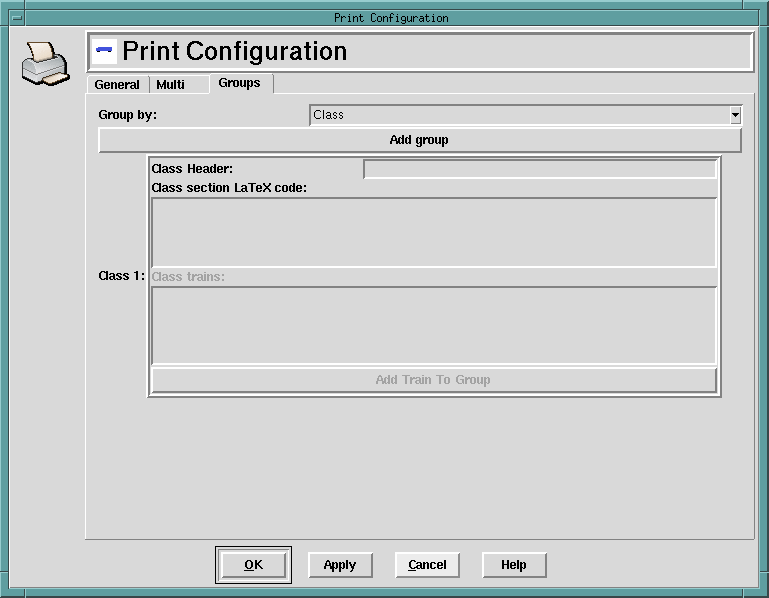
\includegraphics[width=5in]{TTPrintConfigurationDialog3.png}
\caption{Print Configuration dialog, Groups settings}
\label{fig:tt:PrintConfigurationDialog3}
\end{centering}
\end{figure}
The Print Configuration Dialog, shown in
Figures~\ref{fig:tt:PrintConfigurationDialog1};
\ref{fig:tt:PrintConfigurationDialog2}; and
\ref{fig:tt:PrintConfigurationDialog3}, provide for the setting of many
print configuration options. The general settings
(Figure~\ref{fig:tt:PrintConfigurationDialog1}), provide for setting the
title, subtitle, the date, whether to have \LaTeX{} format for double
sided printing, setting the time format, setting the logical direction
of trains, column widths, and including additional commands in the
\LaTeX{} preamble (usually including additional style
packages\footnote{The style pages supertabular and graphicx are already
included.} and style settings). The multi-table settings
(Figure~\ref{fig:tt:PrintConfigurationDialog2}), provide for settings
relating to time tables using multiple tables.  These settings include
whether to create a table of contents, whether to use multiple tables at
all, \LaTeX{} code to precede the table of contents, \LaTeX{} code to
precede notes section, the header to use if a single ``All Trains''
table is generated, and \LaTeX{} code to precede this single ``All
Trains'' table.  The groups settings
(Figure~\ref{fig:tt:PrintConfigurationDialog3}), provide for settings
for each group.  This includes whether to group by class or to manually
group trains and provides for setting the class or group heading and for
\LaTeX{} code to precede the group table, and if grouping manually,
selecting the trains in the group.

\section{Exiting From the Program}

The \texttt{Exit} (or \texttt{Close}) menu item of the \texttt{File}
menu, the 
\includegraphics{TTCloseTool.png} toolbar button, or the
\texttt{Quit -- Exit NOW} button exit the program.  A confirmation
dialog is displayed to get confirmation.

\section{Select One Train Dialog}
\label{sect:tt:SelectOneTrainDialog}

\begin{figure}[hbpt] 
\begin{centering}
\includegraphics{TTSelectOneTrain.png} 
\caption{Select One Train dialog} 
\label{fig:tt:SelectOneTrainDialog} 
\end{centering}
\end{figure} The ``Select One Train dialog'', shown in
Figure~\ref{fig:tt:SelectOneTrainDialog}, is used to select a train
either for deletion (Section~\ref{sect:tt:DeletingTrains}) or for
viewing (Section~\ref{sect:tt:ViewingTrains}).

\section{The View Menu}

The view menu contains menu items for viewing detailed information about
various things, including trains (Section~\ref{sect:tt:ViewingTrains},
stations (Section~\ref{sect:tt:ViewingStations}), and  notes
(Section~\ref{sect:tt:ViewingNotes}).

\subsection{Trains}
\label{sect:tt:ViewingTrains}

There are two menu items for viewing trains, \texttt{View One Train} and
\texttt{View All Trains}.  The \texttt{View One Train} uses the ``Select
One Train dialog'' (Section~\ref{sect:tt:SelectOneTrainDialog}) to
select a train to display detailed information about and the
\texttt{View All Trains} menu item displays a dialog listing all of the
trains, by number and name, with buttons to get more detailed information.

\subsection{Stations}
\label{sect:tt:ViewingStations}

There are two menu items for viewing stations, \texttt{View One
Station} and \texttt{View All Stations}.  The \texttt{View One Station}
uses the ``Select One Station dialog'' to select a station to display
detailed information about and the \texttt{View All Stations} menu item
displays a dialog listing all of the stations, by name and scale mile, with
buttons to get more detailed information.

\subsection{Notes}
\label{sect:tt:ViewingNotes}

There are two menu items for viewing notes, \texttt{View One Note} and
\texttt{View All Notes}.  The \texttt{View One Note} uses the ``Select
One Note dialog'' to select a note to display detailed information
about and the \texttt{View All Notes} menu item displays a dialog
listing all of the notes, by number and beginning text, with buttons to
get more detailed information.

\section{System Configuration}

The Time Table program has a small number of global
configuration options.  These are stored in a file named
\texttt{.timeTable} (\texttt{TimeTable.rc} under MS-Windows) in the
current user's HOME directory.  These configuration options are:
\begin{description}
\item [Path to pdflatex] The pathname to the \texttt{pdflatex}
executable.
\item [Label Width in Chart] The width in pixels of cab, station, and
storage track labels in the time table chart.
\item [Height of main window] The initial height of the main window.
\item [Width of main window] The initial width of the main window.
\end{description}

The system configuration file is read at program startup.  If the
configuration does not exist, a default one is created the first time
the program is run.

The \texttt{Options} menu manages the system configuration, with menu
items to edit the system configuration, save it and reload it.

\section{Add Cab Dialog}
\section{Add Remove Note Dialog}
\section{Create All Cabs Dialog}
\section{Create All Stations Dialog}
\section{Create A New Time Table Dialog}
\section{Edit Note Dialog}
\section{Edit System Configuration}
\section{Edit Train Dialog}
\section{Print Configuration Dialog}
\section{Print Dialog}
\section{Select A Storage Track Name}
\section{Select One Note Dialog}
\section{Select One Station Dialog}
\section{Select One Train Dialog}

\chapter{Help}

This help window contains some basic navigation features.  There are
buttons for traversing the history stack.  There are also key bindings
within the help window itself:

\begin{description}
\item[s] Search forward.  Searches forward in the text for the next
occurance of the specificed text.
\item[r] Search backward.  Searches backward in the text for the next
occurance of the specificed text.
\item[f] History forward.  Goes to the next page in the history stack.
\item[b] History backward. Goes to the previous page in the history
stack.
\item[Tab] Next link. Goes to the next hyperlink.
\item[Control-Tab] Previous link. Goes to the previous hyperlink.
\end{description}




\chapter*{Copying}
\addcontentsline{toc}{chapter}{Copying}
\markboth{Copying}{Copying}
\begin{verbatim}
		    GNU GENERAL PUBLIC LICENSE
		       Version 2, June 1991

 Copyright (C) 1989, 1991 Free Software Foundation, Inc.
     59 Temple Place, Suite 330, Boston, MA  02111-1307  USA
 Everyone is permitted to copy and distribute verbatim copies
 of this license document, but changing it is not allowed.

			    Preamble

  The licenses for most software are designed to take away your
freedom to share and change it.  By contrast, the GNU General Public
License is intended to guarantee your freedom to share and change free
software--to make sure the software is free for all its users.  This
General Public License applies to most of the Free Software
Foundation's software and to any other program whose authors commit to
using it.  (Some other Free Software Foundation software is covered by
the GNU Library General Public License instead.)  You can apply it to
your programs, too.

  When we speak of free software, we are referring to freedom, not
price.  Our General Public Licenses are designed to make sure that you
have the freedom to distribute copies of free software (and charge for
this service if you wish), that you receive source code or can get it
if you want it, that you can change the software or use pieces of it
in new free programs; and that you know you can do these things.

  To protect your rights, we need to make restrictions that forbid
anyone to deny you these rights or to ask you to surrender the rights.
These restrictions translate to certain responsibilities for you if you
distribute copies of the software, or if you modify it.

  For example, if you distribute copies of such a program, whether
gratis or for a fee, you must give the recipients all the rights that
you have.  You must make sure that they, too, receive or can get the
source code.  And you must show them these terms so they know their
rights.

  We protect your rights with two steps: (1) copyright the software, and
(2) offer you this license which gives you legal permission to copy,
distribute and/or modify the software.

  Also, for each author's protection and ours, we want to make certain
that everyone understands that there is no warranty for this free
software.  If the software is modified by someone else and passed on, we
want its recipients to know that what they have is not the original, so
that any problems introduced by others will not reflect on the original
authors' reputations.

  Finally, any free program is threatened constantly by software
patents.  We wish to avoid the danger that redistributors of a free
program will individually obtain patent licenses, in effect making the
program proprietary.  To prevent this, we have made it clear that any
patent must be licensed for everyone's free use or not licensed at all.

  The precise terms and conditions for copying, distribution and
modification follow.
\end{verbatim}
\clearpage
\begin{verbatim}
		    GNU GENERAL PUBLIC LICENSE
   TERMS AND CONDITIONS FOR COPYING, DISTRIBUTION AND MODIFICATION

  0. This License applies to any program or other work which contains
a notice placed by the copyright holder saying it may be distributed
under the terms of this General Public License.  The "Program", below,
refers to any such program or work, and a "work based on the Program"
means either the Program or any derivative work under copyright law:
that is to say, a work containing the Program or a portion of it,
either verbatim or with modifications and/or translated into another
language.  (Hereinafter, translation is included without limitation in
the term "modification".)  Each licensee is addressed as "you".

Activities other than copying, distribution and modification are not
covered by this License; they are outside its scope.  The act of
running the Program is not restricted, and the output from the Program
is covered only if its contents constitute a work based on the
Program (independent of having been made by running the Program).
Whether that is true depends on what the Program does.

  1. You may copy and distribute verbatim copies of the Program's
source code as you receive it, in any medium, provided that you
conspicuously and appropriately publish on each copy an appropriate
copyright notice and disclaimer of warranty; keep intact all the
notices that refer to this License and to the absence of any warranty;
and give any other recipients of the Program a copy of this License
along with the Program.

You may charge a fee for the physical act of transferring a copy, and
you may at your option offer warranty protection in exchange for a fee.

  2. You may modify your copy or copies of the Program or any portion
of it, thus forming a work based on the Program, and copy and
distribute such modifications or work under the terms of Section 1
above, provided that you also meet all of these conditions:

    a) You must cause the modified files to carry prominent notices
    stating that you changed the files and the date of any change.

    b) You must cause any work that you distribute or publish, that in
    whole or in part contains or is derived from the Program or any
    part thereof, to be licensed as a whole at no charge to all third
    parties under the terms of this License.

    c) If the modified program normally reads commands interactively
    when run, you must cause it, when started running for such
    interactive use in the most ordinary way, to print or display an
    announcement including an appropriate copyright notice and a
    notice that there is no warranty (or else, saying that you provide
    a warranty) and that users may redistribute the program under
    these conditions, and telling the user how to view a copy of this
    License.  (Exception: if the Program itself is interactive but
    does not normally print such an announcement, your work based on
    the Program is not required to print an announcement.)
\end{verbatim}
\clearpage
\begin{verbatim}
These requirements apply to the modified work as a whole.  If
identifiable sections of that work are not derived from the Program,
and can be reasonably considered independent and separate works in
themselves, then this License, and its terms, do not apply to those
sections when you distribute them as separate works.  But when you
distribute the same sections as part of a whole which is a work based
on the Program, the distribution of the whole must be on the terms of
this License, whose permissions for other licensees extend to the
entire whole, and thus to each and every part regardless of who wrote it.

Thus, it is not the intent of this section to claim rights or contest
your rights to work written entirely by you; rather, the intent is to
exercise the right to control the distribution of derivative or
collective works based on the Program.

In addition, mere aggregation of another work not based on the Program
with the Program (or with a work based on the Program) on a volume of
a storage or distribution medium does not bring the other work under
the scope of this License.

  3. You may copy and distribute the Program (or a work based on it,
under Section 2) in object code or executable form under the terms of
Sections 1 and 2 above provided that you also do one of the following:

    a) Accompany it with the complete corresponding machine-readable
    source code, which must be distributed under the terms of Sections
    1 and 2 above on a medium customarily used for software interchange; or,

    b) Accompany it with a written offer, valid for at least three
    years, to give any third party, for a charge no more than your
    cost of physically performing source distribution, a complete
    machine-readable copy of the corresponding source code, to be
    distributed under the terms of Sections 1 and 2 above on a medium
    customarily used for software interchange; or,

    c) Accompany it with the information you received as to the offer
    to distribute corresponding source code.  (This alternative is
    allowed only for noncommercial distribution and only if you
    received the program in object code or executable form with such
    an offer, in accord with Subsection b above.)

The source code for a work means the preferred form of the work for
making modifications to it.  For an executable work, complete source
code means all the source code for all modules it contains, plus any
associated interface definition files, plus the scripts used to
control compilation and installation of the executable.  However, as a
special exception, the source code distributed need not include
anything that is normally distributed (in either source or binary
form) with the major components (compiler, kernel, and so on) of the
operating system on which the executable runs, unless that component
itself accompanies the executable.

If distribution of executable or object code is made by offering
access to copy from a designated place, then offering equivalent
access to copy the source code from the same place counts as
distribution of the source code, even though third parties are not
compelled to copy the source along with the object code.
\end{verbatim}
\clearpage
\begin{verbatim}
  4. You may not copy, modify, sublicense, or distribute the Program
except as expressly provided under this License.  Any attempt
otherwise to copy, modify, sublicense or distribute the Program is
void, and will automatically terminate your rights under this License.
However, parties who have received copies, or rights, from you under
this License will not have their licenses terminated so long as such
parties remain in full compliance.

  5. You are not required to accept this License, since you have not
signed it.  However, nothing else grants you permission to modify or
distribute the Program or its derivative works.  These actions are
prohibited by law if you do not accept this License.  Therefore, by
modifying or distributing the Program (or any work based on the
Program), you indicate your acceptance of this License to do so, and
all its terms and conditions for copying, distributing or modifying
the Program or works based on it.

  6. Each time you redistribute the Program (or any work based on the
Program), the recipient automatically receives a license from the
original licensor to copy, distribute or modify the Program subject to
these terms and conditions.  You may not impose any further
restrictions on the recipients' exercise of the rights granted herein.
You are not responsible for enforcing compliance by third parties to
this License.

  7. If, as a consequence of a court judgment or allegation of patent
infringement or for any other reason (not limited to patent issues),
conditions are imposed on you (whether by court order, agreement or
otherwise) that contradict the conditions of this License, they do not
excuse you from the conditions of this License.  If you cannot
distribute so as to satisfy simultaneously your obligations under this
License and any other pertinent obligations, then as a consequence you
may not distribute the Program at all.  For example, if a patent
license would not permit royalty-free redistribution of the Program by
all those who receive copies directly or indirectly through you, then
the only way you could satisfy both it and this License would be to
refrain entirely from distribution of the Program.

If any portion of this section is held invalid or unenforceable under
any particular circumstance, the balance of the section is intended to
apply and the section as a whole is intended to apply in other
circumstances.

It is not the purpose of this section to induce you to infringe any
patents or other property right claims or to contest validity of any
such claims; this section has the sole purpose of protecting the
integrity of the free software distribution system, which is
implemented by public license practices.  Many people have made
generous contributions to the wide range of software distributed
through that system in reliance on consistent application of that
system; it is up to the author/donor to decide if he or she is willing
to distribute software through any other system and a licensee cannot
impose that choice.

This section is intended to make thoroughly clear what is believed to
be a consequence of the rest of this License.
\end{verbatim}
\clearpage
\begin{verbatim}
  8. If the distribution and/or use of the Program is restricted in
certain countries either by patents or by copyrighted interfaces, the
original copyright holder who places the Program under this License
may add an explicit geographical distribution limitation excluding
those countries, so that distribution is permitted only in or among
countries not thus excluded.  In such case, this License incorporates
the limitation as if written in the body of this License.

  9. The Free Software Foundation may publish revised and/or new versions
of the General Public License from time to time.  Such new versions will
be similar in spirit to the present version, but may differ in detail to
address new problems or concerns.

Each version is given a distinguishing version number.  If the Program
specifies a version number of this License which applies to it and "any
later version", you have the option of following the terms and conditions
either of that version or of any later version published by the Free
Software Foundation.  If the Program does not specify a version number of
this License, you may choose any version ever published by the Free Software
Foundation.

  10. If you wish to incorporate parts of the Program into other free
programs whose distribution conditions are different, write to the author
to ask for permission.  For software which is copyrighted by the Free
Software Foundation, write to the Free Software Foundation; we sometimes
make exceptions for this.  Our decision will be guided by the two goals
of preserving the free status of all derivatives of our free software and
of promoting the sharing and reuse of software generally.
\end{verbatim}
\addcontentsline{toc}{section}{Warranty}
\begin{verbatim}
			    NO WARRANTY

  11. BECAUSE THE PROGRAM IS LICENSED FREE OF CHARGE, THERE IS NO WARRANTY
FOR THE PROGRAM, TO THE EXTENT PERMITTED BY APPLICABLE LAW.  EXCEPT WHEN
OTHERWISE STATED IN WRITING THE COPYRIGHT HOLDERS AND/OR OTHER PARTIES
PROVIDE THE PROGRAM "AS IS" WITHOUT WARRANTY OF ANY KIND, EITHER EXPRESSED
OR IMPLIED, INCLUDING, BUT NOT LIMITED TO, THE IMPLIED WARRANTIES OF
MERCHANTABILITY AND FITNESS FOR A PARTICULAR PURPOSE.  THE ENTIRE RISK AS
TO THE QUALITY AND PERFORMANCE OF THE PROGRAM IS WITH YOU.  SHOULD THE
PROGRAM PROVE DEFECTIVE, YOU ASSUME THE COST OF ALL NECESSARY SERVICING,
REPAIR OR CORRECTION.

  12. IN NO EVENT UNLESS REQUIRED BY APPLICABLE LAW OR AGREED TO IN WRITING
WILL ANY COPYRIGHT HOLDER, OR ANY OTHER PARTY WHO MAY MODIFY AND/OR
REDISTRIBUTE THE PROGRAM AS PERMITTED ABOVE, BE LIABLE TO YOU FOR DAMAGES,
INCLUDING ANY GENERAL, SPECIAL, INCIDENTAL OR CONSEQUENTIAL DAMAGES ARISING
OUT OF THE USE OR INABILITY TO USE THE PROGRAM (INCLUDING BUT NOT LIMITED
TO LOSS OF DATA OR DATA BEING RENDERED INACCURATE OR LOSSES SUSTAINED BY
YOU OR THIRD PARTIES OR A FAILURE OF THE PROGRAM TO OPERATE WITH ANY OTHER
PROGRAMS), EVEN IF SUCH HOLDER OR OTHER PARTY HAS BEEN ADVISED OF THE
POSSIBILITY OF SUCH DAMAGES.

		     END OF TERMS AND CONDITIONS
\end{verbatim}
\clearpage
\begin{verbatim}
	    How to Apply These Terms to Your New Programs

  If you develop a new program, and you want it to be of the greatest
possible use to the public, the best way to achieve this is to make it
free software which everyone can redistribute and change under these terms.

  To do so, attach the following notices to the program.  It is safest
to attach them to the start of each source file to most effectively
convey the exclusion of warranty; and each file should have at least
the "copyright" line and a pointer to where the full notice is found.

    <one line to give the program's name and a brief idea of what it does.>
    Copyright (C) <year>  <name of author>

    This program is free software; you can redistribute it and/or modify
    it under the terms of the GNU General Public License as published by
    the Free Software Foundation; either version 2 of the License, or
    (at your option) any later version.

    This program is distributed in the hope that it will be useful,
    but WITHOUT ANY WARRANTY; without even the implied warranty of
    MERCHANTABILITY or FITNESS FOR A PARTICULAR PURPOSE.  See the
    GNU General Public License for more details.

    You should have received a copy of the GNU General Public License
    along with this program; if not, write to the Free Software
    Foundation, Inc., 59 Temple Place, Suite 330, Boston, MA  02111-1307  USA


Also add information on how to contact you by electronic and paper mail.

If the program is interactive, make it output a short notice like this
when it starts in an interactive mode:

    Gnomovision version 69, Copyright (C) year  name of author
    Gnomovision comes with ABSOLUTELY NO WARRANTY; for details type `show w'.
    This is free software, and you are welcome to redistribute it
    under certain conditions; type `show c' for details.

The hypothetical commands `show w' and `show c' should show the appropriate
parts of the General Public License.  Of course, the commands you use may
be called something other than `show w' and `show c'; they could even be
mouse-clicks or menu items--whatever suits your program.

You should also get your employer (if you work as a programmer) or your
school, if any, to sign a "copyright disclaimer" for the program, if
necessary.  Here is a sample; alter the names:

  Yoyodyne, Inc., hereby disclaims all copyright interest in the program
  `Gnomovision' (which makes passes at compilers) written by James Hacker.

  <signature of Ty Coon>, 1 April 1989
  Ty Coon, President of Vice

This General Public License does not permit incorporating your program into
proprietary programs.  If your program is a subroutine library, you may
consider it more useful to permit linking proprietary applications with the
library.  If this is what you want to do, use the GNU Library General
Public License instead of this License.
\end{verbatim}

\include{TimeTable_Version}
\cleardoublepage
\bibliography{MRR}
\bibliographystyle{plain}
\cleardoublepage
\printindex
\end{document}


